%%%%%%%%%%%%%%%%%%%%%%%%%%%%%%% beamer %%%%%%%%%%%%%%%%%%%%%%%%%%%%%%%%%%%%%%%%%%%%%%%%%
% To run - pdflatex filename.tex
%      acroread filename.pdf
%%%%%%%%%%%%%%%%%%%%%%%%%%%%%%%%%%%%%%%%%%%%%%%%%%%%%%%%%%%%%%%%%%%%%%%%%%%%%%%%%%%%%%%%

\documentclass[compress,oilve]{beamer}
\mode<presentation>

\usetheme[]{CambridgeUS}
% other themes: AnnArbor, Antibes, Bergen, Berkeley, Berlin, Boadilla, boxes, CambridgeUS, Copenhagen, Darmstadt, default, Dresden, Frankfurt, Goettingen,
% Hannover, Ilmenau, JuanLesPins, Luebeck, Madrid, Maloe, Marburg, Montpellier, PaloAlto, Pittsburg, Rochester, Singapore, Szeged, classic

\usecolortheme{beaver}
% color themes: albatross, beaver, beetle, crane, default, dolphin,  fly, lily, orchid, rose, seagull, seahorse, sidebartab, whale, wolverine

\usefonttheme{professionalfonts}
% font themes: default, professionalfonts, serif, structurebold, structureitalicserif, structuresmallcapsserif


\hypersetup{pdfpagemode=FullScreen} % makes your presentation go automatically to full screen

% define your own colors:
\definecolor{Red}{rgb}{1,0,0}
\definecolor{Blue}{rgb}{0,0,1}
\definecolor{Green}{rgb}{0,1,0}
\definecolor{magenta}{rgb}{1,0,.6}
\definecolor{lightblue}{rgb}{0,.5,1}
\definecolor{lightpurple}{rgb}{0.8, 0.6, 0.9}
\definecolor{gold}{rgb}{.6,.5,0}
\definecolor{orange}{rgb}{1,0.4,0}
\definecolor{hotpink}{rgb}{1,0,0.5}
\definecolor{newcolor2}{rgb}{.5,.3,.5}
\definecolor{newcolor}{rgb}{0,.3,1}
\definecolor{newcolor3}{rgb}{1,0,.35}
\definecolor{darkgreen1}{rgb}{0, .35, 0}
\definecolor{darkgreen}{rgb}{0, .6, 0}
\definecolor{darkred}{rgb}{.75,0,0}
\definecolor{skyblue}{HTML}{75bbfd}

\definecolor{olive}{cmyk}{0.64,0,0.95,0.4}
\definecolor{purpleish}{cmyk}{0.75,0.75,0,0}

% can also choose different themes for the "inside" and "outside"

% \usepackage{beamerinnertheme_______}
% inner themes include circles, default, inmargin, rectangles, rounded

% \usepackage{beamerouterthemesmoothbars}
% outer themes include default, infolines, miniframes, shadow, sidebar, smoothbars, smoothtree, split, tree


\useoutertheme[subsection=true, height=40pt]{smoothbars}

% to have the same footer on all slides
%\setbeamertemplate{footline}[text line]{STUFF HERE!}
\setbeamertemplate{footline}[text line]{} % makes the footer EMPTY
% include packages
%

%show the page numbers in footnote
%\addtobeamertemplate{navigation symbols}{}{%
%	\usebeamerfont{footline}%
%	\usebeamercolor[fg]{footline}%
%	\hspace{1em}%
%	\insertframenumber/\inserttotalframenumber
%}

\setbeamercolor{footline}{fg=purpleish}
\setbeamerfont{footline}{series=\bfseries}

%add color to curent subsection
\setbeamertemplate{section in head/foot}{\hfill\tikz\node[rectangle, fill=darkred, rounded corners=1pt,inner sep=1pt,] {\textcolor{white}{\insertsectionhead}};}
\setbeamertemplate{section in head/foot shaded}{\textcolor{darkred}{\hfill\insertsectionhead}}

% Remove bullet of subsections
\setbeamertemplate{headline}
{%
	\begin{beamercolorbox}{section in head/foot}
		\insertsectionnavigationhorizontal{\textwidth}{}{}
	\end{beamercolorbox}%
}


% modify headlline, specially headline size
\setbeamertemplate{headline}{%
	\leavevmode%
	\hbox{%
		\begin{beamercolorbox}[wd=\paperwidth,ht=3.5ex,dp=1.125ex]{palette quaternary}%
			\insertsectionnavigationhorizontal{\paperwidth}{}{\hskip0pt plus1filll}
		\end{beamercolorbox}%
	}
}

\setbeamertemplate{footline}{%
	\leavevmode%
	\hbox{\begin{beamercolorbox}[wd=.5\paperwidth,ht=2.5ex,dp=1.125ex,leftskip=.3cm plus1fill,rightskip=.3cm]{author in head/foot}%
			\usebeamerfont{author in head/foot}\insertshortauthor ~ \insertshortinstitute
		\end{beamercolorbox}%
		\begin{beamercolorbox}[wd=.5\paperwidth,ht=2.5ex,dp=1.125ex,leftskip=.3cm,rightskip=.3cm plus1fil]{title in head/foot}%
			\usebeamerfont{title in head/foot}\insertshorttitle\hfill\insertframenumber\,/\,\inserttotalframenumber
	\end{beamercolorbox}}%
	\vskip0pt%
}


%\setbeamertemplate{navigation symbols}{}

\title{Unsupervised Learning: Clustering}
\author{ML Instruction Team, Fall 2022}
\institute[]{CE Department \newline  Sharif University of Technology \newline \newline}
\date[\today]{}
%\titlegraphic{\includegraphics[scale=.35]{example-image}}



%Write \usepackage{etex} just after the \documentclass line (it should be the first loaded package).
\usepackage{etex}
\usepackage{subcaption}
\usepackage{multicol}
\usepackage{physics, amsmath}
\usepackage{epsfig}
\usepackage{graphicx}
\usepackage{amsfonts}
\usepackage{amssymb}
\usepackage[all,knot]{xy}
\xyoption{arc}
\usepackage{url}
\usepackage{multimedia}
\usepackage{hyperref}
\hypersetup{colorlinks,linkcolor=blue,citecolor=redorange,urlcolor=darkred}
\usepackage{multirow}
\usepackage[font={scriptsize}]{caption}
\usepackage{pgf}
\usepackage{fontspec}
\usepackage{subcaption}
\usepackage[export]{adjustbox}
\usepackage{caption}
%\setsansfont[Scale=MatchLowercase, BoldFont = * Bold, ItalicFont = * Italic]{Caladea}
\graphicspath{ {./Pictures/} }
%\usepackage{enumitem,xcolor}
%\newcommand{\labelitemi}{$\blacksquare$}
%\newcommand{\labelitemii}{$\diamond$}
%\newcommand{\labelitemiii}{$\square$}
%\newcommand{\labelitemiv}{$\ast$}
%\setbeamercolor*{item}{fg=red}
\usepackage{bm}

\usefonttheme{professionalfonts} 
\setbeamertemplate{itemize item}{\color{skyblue}$\blacksquare$}
\setbeamertemplate{itemize subitem}{\color{hotpink}$\blacktriangleright$}
\setbeamertemplate{itemize subsubitem}{\color{orange}$\bullet$}


\usepackage{anyfontsize}
\usepackage{t1enc}
\usepackage{tikz}
\usetikzlibrary{calc,trees,positioning,arrows,chains,shapes.geometric,decorations.pathreplacing,decorations.pathmorphing,shapes,matrix,shapes.symbols}


\DeclareMathOperator*{\argmin}{argmin}
\newtheorem{proposition}[theorem]{Proposition}
\newtheorem{remark}[theorem]{Remark}
\newtheorem{assumption}[theorem]{Assumption}

\usepackage{fontspec,unicode-math}
\setmainfont[Scale=0.9]{Consolas}
\setmonofont[Scale=0.9]{Monaco}
\setsansfont[Scale=1]{Times New Roman}
\newcommand{\vect}[1]{\boldsymbol{#1}}


%\usepackage{smartdiagram}
%\usesmartdiagramlibrary{additions}
%%%%%%%%%%%%%%%%%%%%%%%%%%%%%%%%%%%%%%%%%%%%%%%%%%%%%%%%%%%%%%%%%%%%%%%%%%%%%%%%%%%%%%%%%%%%
%%%%%%%%%%%%%%%%%%%%%%%%%%%%%% Title Page Info %%%%%%%%%%%%%%%%%%%%%%%%%%%%%%%%%%%%%%%%%%%
%%%%%%%%%%%%%%%%%%%%%%%%%%%%%%%%%%%%%%%%%%%%%%%%%%%%%%%%%%%%%%%%%%%%%%%%%%%%%%%%%%%%%%%%%%


%%%%%%%%%%%%%%%%%%%%%%%%%%%%%%%%%%%%%%%%%%%%%%%%%%%%%%%%%%%%%%%%%%%%%%%%%%%%%%%%%%%%%%%%%%
%%%%%%%%%%%%%%%%%%%%%%%%%%%%%% Begin Your Document %%%%%%%%%%%%%%%%%%%%%%%%%%%%%%%%%%%%%%%
%%%%%%%%%%%%%%%%%%%%%%%%%%%%%%%%%%%%%%%%%%%%%%%%%%%%%%%%%%%%%%%%%%%%%%%%%%%%%%%%%%%%%%%%%%
\begin{document}
	
%%%%%%%%%%%%%%%%%%%%%%%%%%%%%%%%%%%%%%%%%%%%%%%%%%%%%%%%%%%%%%%%%%%%%%%%%%%%%%%%%%%%%%%%%%
	\fontsize{9}{9}
\begin{frame}[noframenumbering, plain]
	\titlepage
\end{frame}

%%%%%%%%%%%%%%%%%%%%%%%%%%%%%%%%%%%%%%%%%%%%%%%%%%%%%%%%%%%%%%%%%%%%%%%%%%%%%%%%%%%%%%%%%%
\section{Introduction}
%%%%%%%%%%%%%%%%%%%%%%%%%%%%%%%%%%%%%%%%%%%%%%%%%%%%%%%%%%%%%%%%%%%%%%%%######

%%%%%%%%%%%%%%%%%%%%%%%%%%%%%%%%%%%%%%%%%%%%%%%%%%%%%%%%
\begin{frame}{Clustering: An Overview}
\begin{itemize}
\item Clustering algorithms can be classified into different categories, based on the following criteria:
	\begin{itemize}
		\item Whether each point is assigned to exactly one cluster or several clusters with certain probabilites that add up to 1:
			\begin{itemize}
				\item \textbf{Hard}
				\item \textbf{Soft}
			\end{itemize}
		\item Whether all clusters are on the same level or several clusters are built in a hierarchical way:
			\begin{itemize}
				\item \textbf{Partitional}
				\item \textbf{Hierarchical}
			\end{itemize}
	\end{itemize}
\end{itemize}
\begin{columns}
	\begin{column}{0.5\textwidth}
		\begin{figure}
			 \centering
			 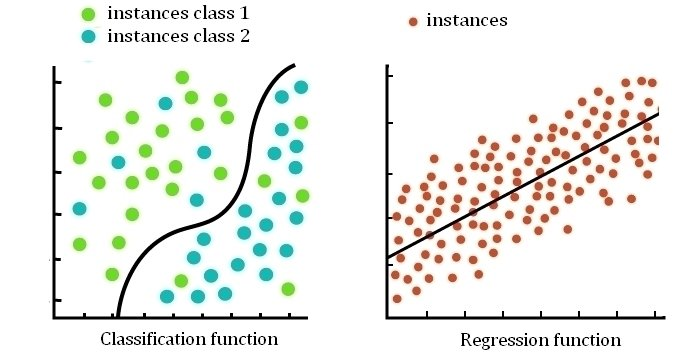
\includegraphics[scale=0.45]{3} 
			 \caption{Hard vs Soft [1].}
		\end{figure}
	\end{column}
	\begin{column}{0.5\textwidth}
		\begin{figure}
			 \centering
			 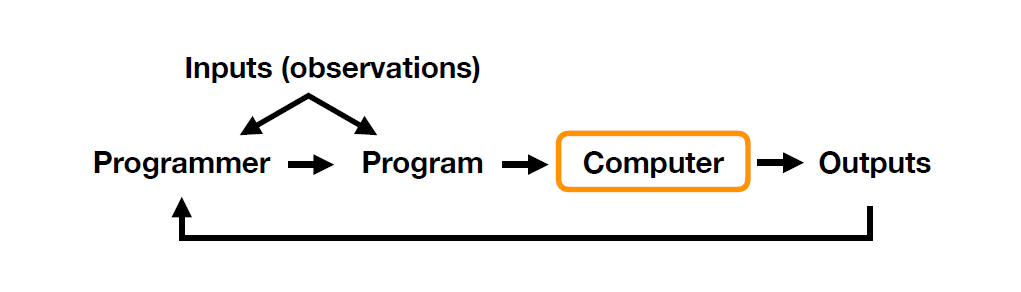
\includegraphics[scale=0.45]{1}  
 			 \caption{Partitional vs Heirarchical [2].}
		\end{figure}
	\end{column}
\end{columns}
\end{frame}

\begin{frame}{Clustering: An Overview}
\begin{itemize}
\item Hierarchical clustering is usually done in two different ways:
	\begin{itemize}
		\item \textbf{Agglomerative}: This is a "bottom-up" approach, Each observation starts in its own cluster, and pairs of clusters are merged as one moves up the hierarchy.
		\item \textbf{Divisive}: This is a "top-down" approach, All observations start in one cluster, and splits are performed recursively as one moves down the hierarchy.
	\end{itemize}
\end{itemize}
\begin{figure}
	\centering
	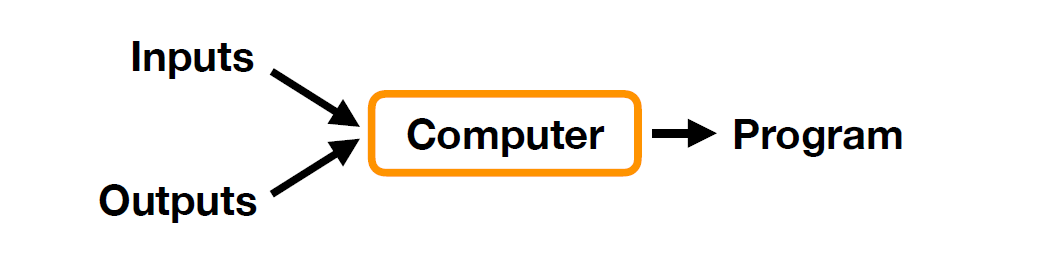
\includegraphics[scale=0.35]{2}
	\caption{Agglomerative vs Divisive [3].}
\end{figure}
\end{frame}


\begin{frame}{Hard Partitional Clustering: $K$-Means}
\begin{itemize}
\item A particularly simple method for clustering is $K$-means, The idea is \textbf{to represent each cluster $ k $ by a center point $\mathbf{c_{\mathnormal k}} $ and assign each data point $ \mathbf{x_{\mathnormal n}}$ to one of the clusters $ k $} which can be written in terms of index sets $\mathcal{C_{k}}$
\item The center points and the assignment are then chosen such that the mean squared distance between data points and center points \textbf{is minimized}:
$$ J := \displaystyle\sum_{n=1}^{N} \displaystyle\sum_{k=1}^{K} r_{nk} \| \mathbf{x_{\mathnormal n}} -  \mathbf{c_{\mathnormal k}} \| ^ {2} $$
\item Here we introduced a corresponding binary indicator variable $ r_{nk} \in \{0, 1\} $ where $ k = 1, 2, \dots, K $ describing which of the $ K $ clusters the data point $ \mathbf{x_{n}} $ is assigned to, so that if data point  $ \mathbf{x_{n}} $ is assigned to cluster $ k $ then $ r_{nk} = 1$, and $ r_{nj} = 0 $ for $ j \neq k $
\item Now, Our goal is to find values for the $\{r_{nk}\}$ and the $ \{\mathbf c_{k}\}$ so as to minimize $ J $. we can do this through an \textbf{Iterative Procedure}
\end{itemize}
\end{frame}


\begin{frame}{Hard Partitional Clustering: $K$-Means}
\begin{itemize}
\item To minimize $ J $ through iterating, we have to do the following algorithm :
	\begin{enumerate}
		\item \textbf{Initialize} $ \mathbf{c_{k}} $ with \textbf{Random Value} for all $ k = 1, 2, \dots, K$, It could be chosen from data values either.
		\item Minimize $ J $ with respect to $ r_{nk} $, keeping the $ c_{k} $ fixed. because $ J $ is a linear function of $ r_{nk} $ this optmization can be performed easily to give a closed form solution:
				$$ r_{nk} = \begin{cases}
    1      & \quad \text{if } k =  \argmin_{j} \| \mathbf{x_{\mathnormal n}} -  \mathbf{c_{\mathnormal j}} \| ^ {2}\\
    0  & \quad \text{otherwise}
  \end{cases} $$
		\item Minimize $ J $ with respect to $ \mathbf{c_{k}} $, keeping the $ r_{nk} $ fixed. if the assignment is fixed, it is easy to show that the optimal choice of the center positions is given by:
			$$ \mathbf{c_{k}} =  \frac{\sum_{n} r_{nk}\mathbf x_{\mathnormal n}}{\sum_{n} r_{nk}}$$
		\item Check the convergence criteria, otherwise go to step 2.	
	\end{enumerate}
\end{itemize}
\end{frame}

\begin{frame}{Hard Partitional Clustering: $K$-Means}
\begin{figure}
	\centering
	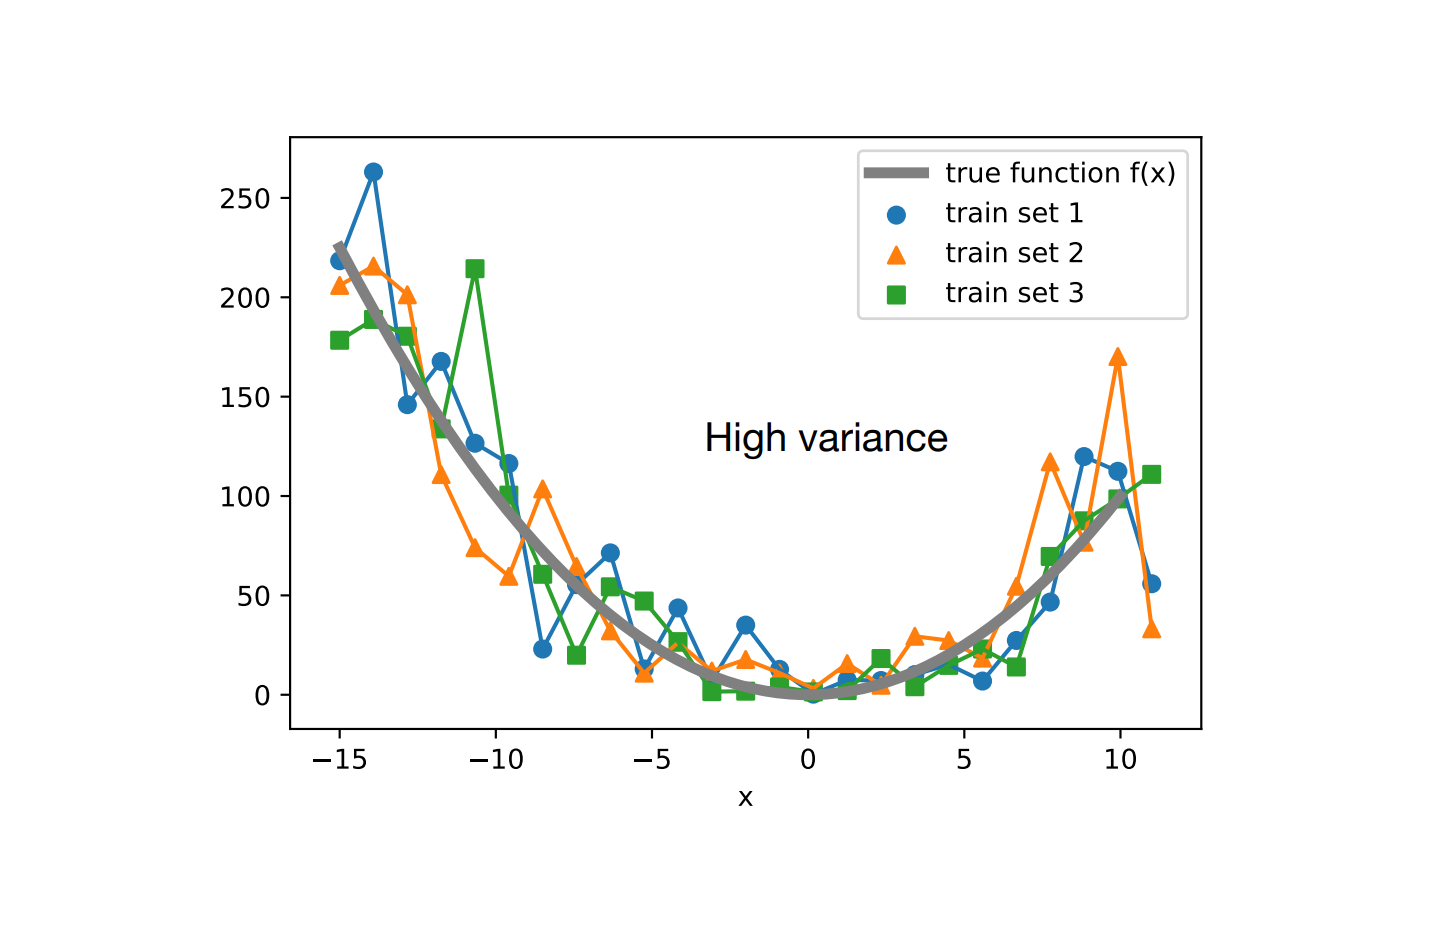
\includegraphics[scale=0.5]{8}
	\caption{Illustration of $K$-Means with $K = 2$}
\end{figure}
\end{frame}

\begin{frame}{Hard Partitional Clustering: $K$-Means}
\begin{itemize}
\item Note that the result of the algorithm is \textbf{not necessarily a global optimum} of the objective function $ J $
\item It is therefore advisable to \textbf{run the algorithm several times} with different initial center locations and \textbf{pick the best result}.
\item A drawback of this and many other clustering algorithms is that \textbf{the number of clusters is not determined}.
\item One has to decide on a proper $K$ in advance, or one simply runs the algorithm with several different $K$-values and picks the best according to some criterion.
\end{itemize}
\end{frame}





%\begin{frame}{Machine Learning: An Overview}
%\begin{itemize}
%\item[$\blacksquare$] Among these quotions that we have discussed, one seems more interesting and important:\\
%\begin{center} \textit{"Machine learning is the field of study that gives computers the ability to
%learn without being explicitly programmed”} \\ 
%— Arthur L. Samuel, AI pioneer, 1959 \end{center}
%\item[$\blacksquare$] But why does it seem important? why should computers be able to learn? waht do they really learn? \\
%\item[$\blacksquare$] We shall answer these questions through this lecture
%\end{itemize}
%\end{frame}





%\begin{frame}{Machine Learning: An Overview}
%\begin{itemize}
%\item The preceding traditional programming paradigm has several disadvantages:
%	\begin{itemize}
%	\item what if we don't know waht program should we write for the given data (inputs) ?
%	\item what if the inputs change dynamically over the time? should we write another program? 
%	\end{itemize}
%\item In order to resolve such problems, we should replace the need of developing computer programs "manually"
%\item In other words, we would like to automate the process of creating programs by informing the computer, the inputs and outputs that it needs:
%\begin{center}
%\begin{figure}
%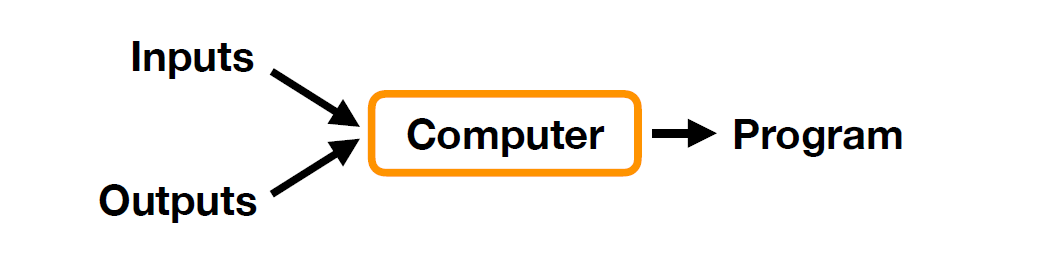
\includegraphics[scale=0.5]{2}
%\center \caption{ML Paradigm [1].}
%\end{figure}
%\end{center}
%\end{itemize}
%\end{frame}


%%%%%%%%%%%%%%%%%%%%%%%%%%%%%%%%%%%%%%%%%%%%%%%%%%%%%%%%%%%%%%%%%%%%%%%%%%%%%%%%%%%%%%%%%%%%%%%

%%%%%%%%%%%%%


%\begin{frame}{Categories of Machine Learning}
%\begin{itemize}
%\item The three broad categories of ML are summerized in:
%\begin{itemize}
%\item \textbf{Supervised Learning}
%\item \textbf{Unsupervised Learning}  
%\item \textbf{Reinforcement Learning} 
%\end{itemize}
%\end{itemize}
%\begin{figure}
%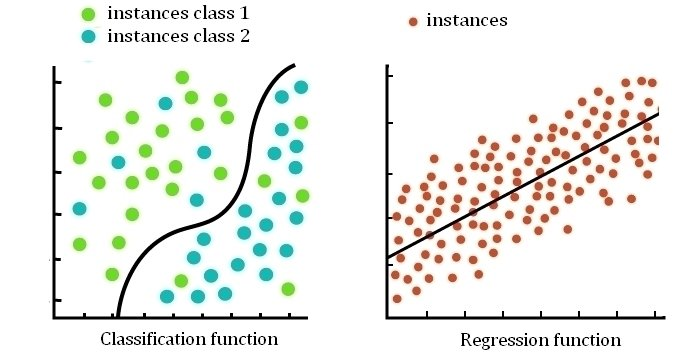
\includegraphics[scale=0.5, right]{3}
%\caption{Categories of ML [2].}
%\end{figure}
%\end{frame}



%\begin{frame}{Unsupervised Learning}
%\begin{itemize}
%\item In contrast to supervised learning, unsupervised learning is a branch of machine learning that is concerned with unlabeled data. Common tasks in unsupervised learning are \textbf{Clustering} analysis and \textbf{Dimensionality Reduction}.
%\end{itemize}
%\begin{columns}
%\begin{column}{0.4\textwidth}
%\begin{figure}
% \centering
% 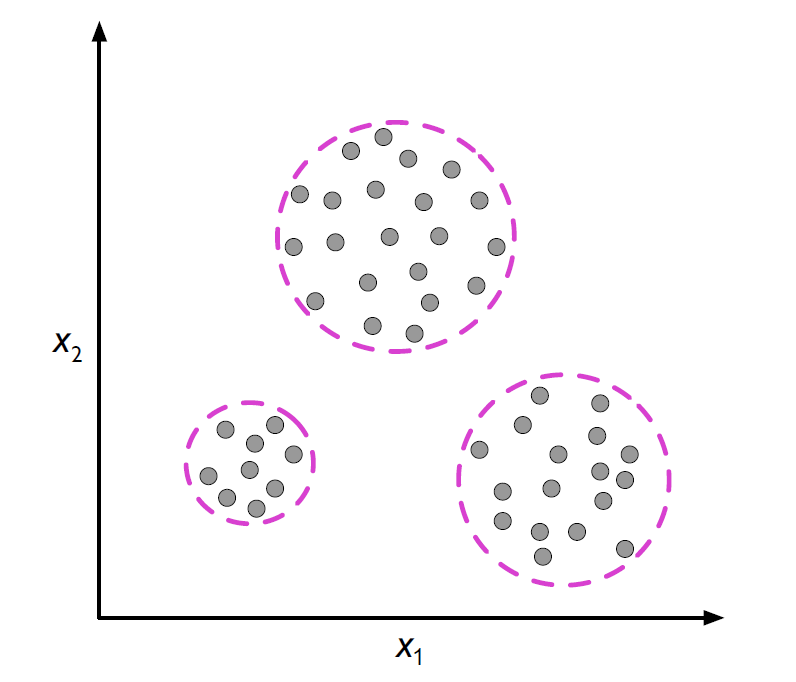
\includegraphics[scale=0.25]{14}  
% \caption{Illustration of Clustering [2].}
%\end{figure}
%\end{column}
%\begin{column}{0.6\textwidth}
%\begin{figure}
% \centering
% 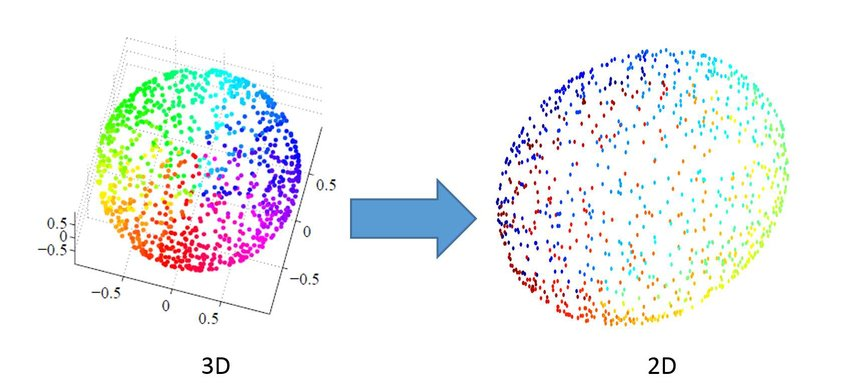
\includegraphics[scale=0.25]{16}  
 %\caption{Illustration of Dimensionality Reduction [3].}
%\end{figure}
%\end{column}
%\end{columns}
%\end{frame}



%\begin{frame}{5 Steps To Solve A Machine Learning Problem}
%\begin{itemize}
%\item 1. Define the problem to be solved.
%\item 2. Collect (labeled) data.
%\item 3. Choose an algorithm class.
%\item 4. Choose an optimization metric for learning the model.
%\item 5. Choose a metric for evaluating the model.
%\end{itemize}
%\begin{figure}
 %\centering
% 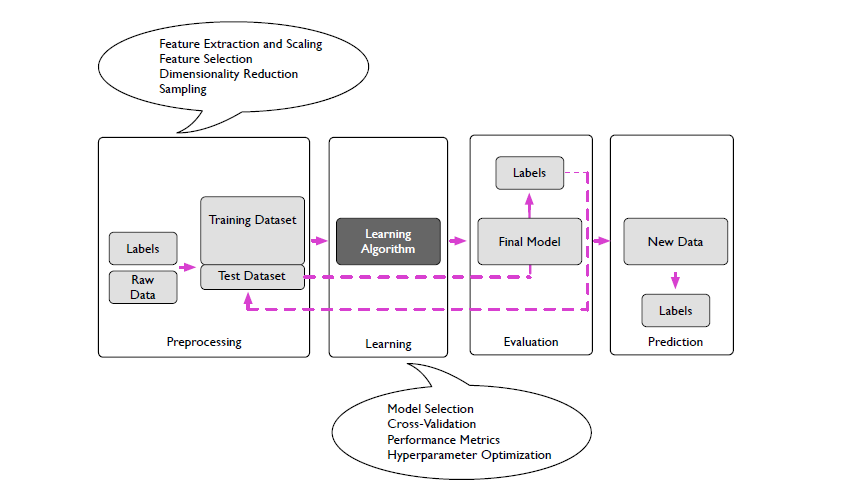
\includegraphics[scale=0.6]{13}  
% \caption{Learning Process [2].}
%\end{figure}
%\end{frame}


%\begin{frame}{Optimization Methods}
%\begin{columns}
%\begin{column}{0.5\textwidth}
%\begin{itemize}
%\item Combinatorial search, greedy search (e.g., decision trees over, not within nodes);
%\item Unconstrained convex optimization (e.g., logistic regression);
%\item Constrained convex optimization (e.g., SVM);
%\item Nonconvex optimization, here: using backpropagation, chain rule, reverse autodi. (e.g., neural networks).
%\item Constrained nonconvex optimization (semi-adversarial networks, not covered in this course)
%\end{itemize}
%\end{column}
%\begin{column}{0.5\textwidth}
%\begin{figure}
%\centering
%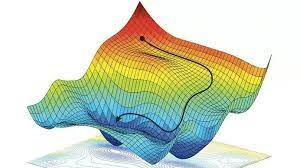
\includegraphics[scale=0.35]{17}  
 %\caption{Gradient Descent [10].}
%\end{figure}
%\begin{figure}
%\centering
%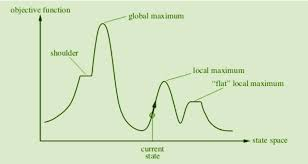
\includegraphics[scale=0.35]{26}  
% \caption{Hill Climbing [11].}
%\end{figure}
%\end{column}
%\end{columns}
%\end{frame}



%%%%%%%%%%%%%%%%%%%%%%%%%%%%%%



\begin{frame}{References}
\begin{itemize}
\item{} \textbf{[1]}. Raschka, Sebastian. “What Are Data Science and Machine Learning?” Dr. Sebastian Raschka, 3 Sept. 2022, sebastianraschka.com/faq/docs/datascience-ml.html.
\item{} \textbf{[2]}. Raschka, Sebastian, and Vahid Mirjalili. Python Machine Learning: Machine Learning and Deep Learning With Python, Scikit-learn, and TensorFlow 2, 3rd Edition. 3rd ed., Packt Publishing, 2019.
\item{} \textbf{[3]}. Peluffo, Diego. Dimensionality Reduction Effect Over an Artificial (3-dimensional) Spherical Shell Manifold. Resultant Embedded (2-dimensional) Data Is an Attempt to Unfolding the Original Data. Feb. 2017, www.researchgate.net/publication 313787026-Interactive-Data-Visualization-Using-Dimensionality-Reduction-and-Similarity-Based-Representations.
\item{} \textbf{[4]}. Kumar, Ajitesh. “5 Common Ensemble Methods in Machine Learning.” Data Analytics, 16 Aug. 2022, vitalflux.com/5-common-ensemble-methods-in-machine-learning.
\item{} \textbf{[5]}. http://strijov.com/sources/demo-GLM.php
\item{} \textbf{[6]}. www.researchgate.net/figure/Schematic-of-a-Decision-Tree-The-figure-shows-an-example-of-a-decision-tree-with-3-fig1-348456545. Accessed 8 Sept. 2022.
\end{itemize}
\end{frame}


\begin{frame}{References}
\begin{itemize}
\item{} \textbf{[7]}. Wikipedia contributors. “Support-vector Machine.” Wikipedia, 1 Sept. 2022, en.wikipedia.org/wiki/Support-vector-machine.
\item{} \textbf{[8]}. www.researchgate.net/figure/Simple-directed-graphical-model-with-three-variables-To-illustrate-how-graphical-models-fig6-262407302. Accessed 8 Sept. 2022.
\item{} \textbf{[9]}. Ashtari, Hossein. “What Is a Neural Network? Definition, Working, Types, and Applications in 2022.” Spiceworks, 3 Aug. 2022, www.spiceworks.com/tech/artificial-intelligence/articles/what-is-a-neural-network.
\item{} \textbf{[10]}. Balaouras, Georgios. “Optimization Algorithms.” Georgios Balaouras, 21 Apr. 2022, mpalaourg.me/project/optimization-algorithms.
\item{} \textbf{[11]}. GeeksforGeeks. “Introduction to Hill Climbing | Artificial Intelligence.” GeeksforGeeks, 23 Aug. 2022, www.geeksforgeeks.org/introduction-hill-climbing-artificial-intelligence.
\item{} \textbf{[12]}. Agrawal, Sanidhya. “What Is Instance-Based Learning? - Sanidhya Agrawal.” Medium, 14 Dec. 2021, medium.com/@sanidhyaagrawal08/what-is-instance-based-learning-a9b06079e836.
\end{itemize}
\end{frame}


\frametitle{Final Notes}
\centering
\vspace{50 pt}
\textbf{Thank You!}
\vspace{50pt}

\textbf{Any Question?}
%%%%%%%%%%%%%%%%%%%%%%%%%%%%%%%%%%%%%%%%%%
\end{document}